\section{Gaussian Processes}
\begin{framed}
    A Gaussian process is characterized by a \textbf{mean function} $\mu : \spX \to \R$ and a \textbf{covariance function} (or \textbf{kernel function}) $k : \spX \times \spX \to \R$ such that for any $\sA \defeq \{\vx_1, \dots, \vx_m\} \subseteq \spX$, we have 
  $\vf_\sA \defeq \transpose{[f_{\vx_1} \; \cdots \; f_{\vx_m}]} \sim \N{\vmu_\sA}{\mK_{\sA\sA}}$ 
We write $f \sim \GP{\mu}{k}$.
In particular,  
  $\ys \mid \vxs, \mu, k \sim \N{\mu(\vxs)}{k(\vxs, \vxs) + \sigman^2}$ (homoscedastic noise)
\end{framed}
\begin{framed}
    \textbf{Maximize Marginal Likelihood}: \\
    $ \vthetahat_\MLE \defeq \argmax_{\vtheta} p(y_{1:n} \mid \vx_{1:n}, \vtheta) \\= \argmax_{\vtheta} \int p(y_{1:n} \mid \vx_{1:n}, f, \vtheta) p(f \mid \vtheta) \,d f$.
\end{framed}
\textbf{Update:} Joint distribution of the observations $y_{1:n}$ and the noise-free prediction $\fs$ at a test point $\vxs$ as $\begin{bmatrix}
    \vy \\
    \fs \\
  \end{bmatrix} \mid \vxs, \vx_{1:n} \sim \N{\Tilde{\vmu}}{\Tilde{\mK}}$ \\
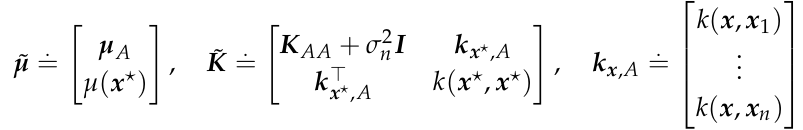
\includegraphics[width=\linewidth]{images/GP_Update}
\textbf{GP posterior}: 
$f \mid \vx_{1:n}, y_{1:n} \sim \GP{\mu'}{k'}$ where $
  \mu'(\vx) \defeq \mu(\vx) + \transpose{\vk_{\vx,\sA}} \inv{(\mK_{\sA\sA} + \sigman^2 \mI)} (\vy_\sA - \vmu_\sA)$ and $
  k'(\vx, \vxp) \defeq k(\vx, \vxp) - \transpose{\vk_{\vx,\sA}} \inv{(\mK_{\sA\sA} + \sigman^2 \mI)} \vk_{\vxp,\sA}$
For GP-Regression ($y_{1:n} \mid \vx_{1:n}, \vtheta \sim \N{\vzero}{\mK_{f,\vtheta} + \sigman^2 \mI}$), write $\mK_{\vy,\vtheta} \defeq \mK_{f,\vtheta} + \sigman^2 \mI$, and obtain: $\vthetahat_\MLE = \argmin_{\vtheta} \frac{1}{2} \transpose{\vy} \inv{\mK_{\vy,\vtheta}} \vy + \frac{1}{2} \log \det{\mK_{\vy,\vtheta}}$. Also:
$\pdv{}{\theta_j} \log p(y_{1:n} \mid \vx_{1:n}, \vtheta) = \frac{1}{2} \tr{(\valpha \transpose{\valpha} - \inv{\mK_{\vy,\vtheta}}) \pdv{\mK_{\vy,\vtheta}}{\theta_j}}$.\\
\textbf{Approximations}: Gaussian process need to invert Matrices $\rightarrow$ computational cost of $\BigO{n^3}$. \\ 
\textbf{Local method}: When sampling at $\vx$ only condition on the samples $\vxp$, that are close, i.e. where $\abs{k(\vx, \vxp)} \geq \tau$ for some $\tau > 0$, instead of all samples. \textbf{Problem:} $\tau$ has to be chosen carefully: if $\tau$ is chosen too large, samples become essentially independent. \\
\textbf{Kernel Approximation}: Construct a low dimensional feature map $\vphi : \R^d \to \R^m$ that approximates the kernel: $k(\vx, \vxp) \approx \transpose{\vphi(\vx)} \vphi(\vxp)$. Then apply Bayesian linear regression $\rightarrow$ time complexity of $\BigO{n m^2 + m^3}$. This can be done with \textbf{Random Fourier features}: a \textit{stationary} kernel $k$ can be interpreted as a function in one variable, and has an associated Fourier transform which we denote by $p(\vomega)$: $k(\vx-\vxp) = \int_{\R^d} p(\vomega) e^{i \transpose{\vomega} (\vx-\vxp)} \,d\vomega$.
\begin{framed}
    \textbf{Bochner's Theorem} A continuous Kernel on $\R^d$ is p.s.d iff its Fourier transform $p(\vomega)$ is non-negative.
\end{framed}
$\implies$ If continuous and stationary kernel is p.s.d. and scaled correctly then $p(\vomega)$ is a probability distribution named \textbf{spectral density} of $k$. The spectral density can be computed by: $p(\vomega) = \int_{\R^d} k(\vomega) e^{- i 2 \pi \transpose{\vxi} \vomega} \,d\vomega.$ \\ Now write the kernel as an expectation: $k(\vx-\vxp) = \int_{\R^d} p(\vomega) e^{i \transpose{\vomega} (\vx-\vxp)} \,d\vomega = \E[\vomega \sim p]{e^{i \transpose{\vomega}(\vx-\vxp)}}= \transpose{\vz(\vx)} \vz(\vxp)$, where $z_{\vomega,b}(\vx) \defeq \sqrt{2} \cos(\transpose{\vomega} \vx + b)$, and $\vz(\vx) \defeq \frac{1}{\sqrt{m}} \transpose{[z_{\vomega^{(1)},b^{(1)}}(\vx), \dots, z_{\vomega^{(m)},b^{(m)}}(\vx)]}$ is a randomized feature map of Fourier transforms $\vomega^{(i)} \iid p$ and $b^{(i)} \iid \Unif{\brackets{0, 2 \pi}}$. The error probability decays exponentially in $\epsilon$.
\begin{framed}
    \textbf{Inducing Points}    
    SoR/FITC: runtime \(\mathcal{O}(n^3)\) in number of inducing points, \(\mathcal{O}(n)\) in number of points. Inducing points can be seen as hyperparameters to optimize.
\end{framed}
